\documentclass{article}

\usepackage{iclr2026_conference,times}
\input{math_commands.tex}

\usepackage{amsmath}
\usepackage{amssymb}
\usepackage{amsthm}
\usepackage{graphicx}
\usepackage{booktabs}
\usepackage{array}
\usepackage{url}
\usepackage{xcolor}
\usepackage[hypertexnames=false]{hyperref}

\graphicspath{{../figures/}}

\newtheorem{proposition}{Proposition}
\newcommand{\score}{S}
\newcommand{\utility}{R}
\newcommand{\pool}{\mathcal{D}}
\newcommand{\Expect}{\mathbb{E}}
\newcommand{\rssm}{RSSM}

\title{\raggedright Belief-Tail Audits for RSSM World Models:\\Diagnosing Latent Imagination Failures Before Execution}

\author{Anonymous Authors}

\begin{document}
\maketitle

\begin{abstract}
RSSM world models plan in latent space, where the highest-valued imagined trajectory can be a model artifact rather than an executable plan. We study this failure as a belief-tail problem: before execution, the selected high-score tail should be audited for posterior-prior drift, decoder inconsistency, hidden-mode belief collapse, and pilot-calibrated latent-real disagreement. The paper proposes a leakage-audited belief-tail protocol that measures selected-tail utility on empirical candidate pools, diagnoses when latent score and executed utility separate, and applies architecture-aware repair scores. Controlled hidden-mode dynamics, a small CPU-trained \rssm-style model, belief-intervention stress tests, receding-horizon planning, out-of-distribution stress grids, label-budget ablations, three lightweight Gymnasium toy-text benchmarks, and three standard Gymnasium classic-control tasks show that raw large-candidate planning can raise imagined value while executed utility stagnates or decreases in diagnosed regimes. Diagnostic repairs recover substantial selected-tail utility without claiming full Dreamer validation, broad model-based-RL coverage, or robotics evidence.
\end{abstract}

\section{Introduction}

World models make planning attractive because an agent can evaluate many imagined futures before acting. In latent model-based reinforcement learning, including recurrent state-space model (\rssm) agents such as PlaNet and Dreamer \citep{hafner2019planet,hafner2020dreamer,hafner2021dreamerv2,hafner2023dreamerv3}, this planning step often samples or optimizes candidate action sequences, scores them under the learned latent model, and executes the candidate with the largest imagined return. More candidates reliably improve the selected latent score. The harder question is whether the selected action remains executable in the real hidden dynamics.

This paper studies that question as a belief-tail audit problem. The failure is not simply that the model is wrong on average. The dangerous case is concentrated in the selected high-score tail: ambiguous observations, stochastic latent priors, and hidden execution modes can make a trajectory look plausible under imagined belief while its realized utility is poor. In this regime, a larger candidate budget can become a search procedure for model artifacts. The selected imagined value rises, but the executed utility stagnates or falls.

Our contribution is a compact audit protocol for \rssm-style latent imagination. First, we define belief-tail diagnostics that are available before execution: posterior-prior drift, decoder/state inconsistency, uncertainty, and hidden-mode belief collapse. Second, we evaluate whether those diagnostics predict the selected-tail latent-real gap across analytic hidden-mode rollouts, a small learned \rssm-style model, receding-horizon planning, label-budget calibration, OOD stress regimes, three toy-text Gymnasium benchmarks, and three standard Gymnasium classic-control tasks. Third, we test leakage-audited repair scores that use only disjoint pilot labels and architecture-aware penalties. A finite selected-tail estimator is used as a measurement device throughout; it is not presented as the paper's novelty or as a new planning algorithm.

The main finding is conditional and deliberately bounded. In these CPU-scale settings, raw large-candidate latent planning often amplifies selected-tail errors, while RSSM-aware diagnostics recover a substantial fraction of the oracle gap without erasing all risk. The evidence does not claim full Dreamer validation, broad model-based-RL coverage, or robotics readiness.

\section{Belief-Tail Measurement Protocol}

Consider a finite empirical pool \(\pool=\{(\score_i,\utility_i)\}_{i=1}^m\), where \(\score_i\) is the score used for selection and \(\utility_i\) is the measured utility we care about. In our experiments \(\score_i\) is usually an imagined latent return or a repaired latent score, while \(\utility_i\) is the utility obtained by executing the action sequence in the hidden-mode environment. A candidate-budget selector draws \(N\) candidates independently with replacement from \(\pool\), selects a draw with maximum score, and breaks score ties uniformly among the tied top-score draws.

Sort candidates by score in ascending order. Let score tie group \(g\) occupy 1-indexed rank interval \([r_g^{\min}, r_g^{\max}]\), and let \(\bar{\utility}_g\) be the mean measured utility of candidates in that tie group.

\begin{proposition}[Finite selected-tail estimator]
\label{prop:tail-estimator}
For any candidate budget \(N\geq 1\), the expected measured utility selected by the highest-score candidate is
\begin{equation}
\label{eq:tail-estimator}
\Expect[\utility_{\mathrm{sel}}(N)]
= \sum_g \bar{\utility}_g
\left[
\left(\frac{r_g^{\max}}{m}\right)^N
- \left(\frac{r_g^{\min}-1}{m}\right)^N
\right].
\end{equation}
\end{proposition}

The bracketed term is exactly the probability that the maximum sampled score lies in tie group \(g\). Conditional on that event, uniform tie-breaking makes the selected utility equal to the tie group's mean utility. The proof is included in Appendix~\ref{app:proof}. The estimator makes no assumption that scores are calibrated, monotone, or useful. If score and measured utility are aligned in the selected tail, larger candidate budgets improve utility. If they are anti-aligned, larger budgets worsen utility. The audit target is latent-real mismatch: the selected latent score \(\Expect[\score_{\mathrm{sel}}(N)]\) increases with \(N\), while \(\Expect[\utility_{\mathrm{sel}}(N)]\) is flat or decreases. Figure~\ref{fig:theory-main} validates the estimator against Monte Carlo simulation and shows aligned, constant, and anti-aligned regimes.

\begin{figure}[t]
  \centering
  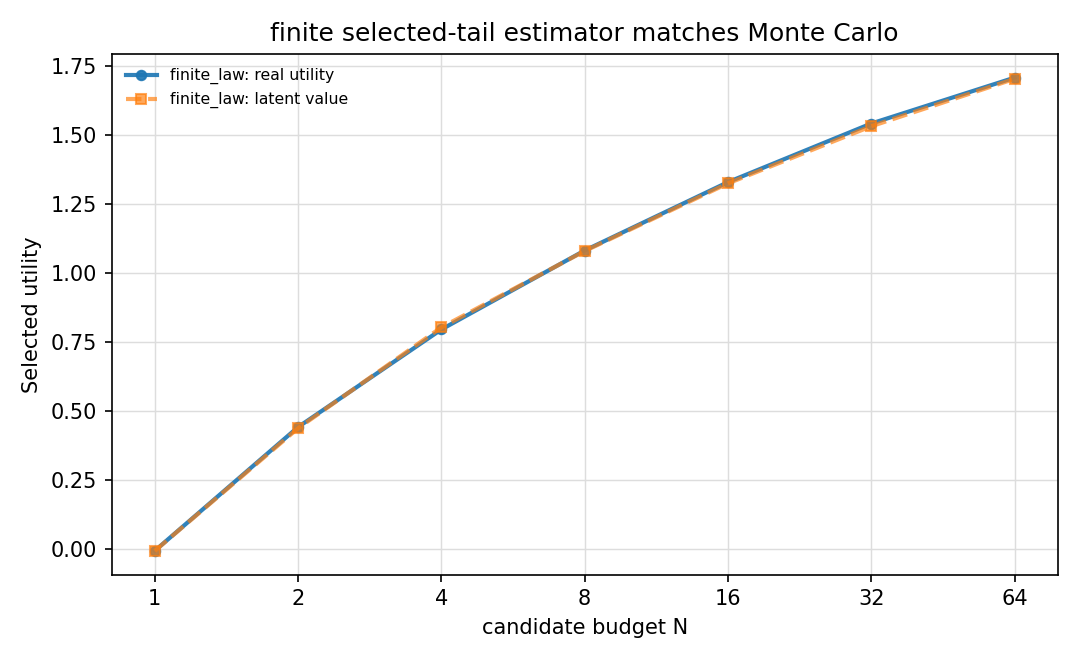
\includegraphics[width=0.82\linewidth]{figure5_selected_tail_estimator.png}
  \caption{The finite selected-tail estimator exactly predicts selected utility curves from empirical candidate pools. Monte Carlo error is below \(0.01\) in this validation. Oracle scoring improves selected utility with \(N\), constant utility remains constant, and anti-aligned scoring degrades utility.}
  \label{fig:theory-main}
\end{figure}

\section{RSSM-Style Candidate Scoring and Repair}

At a planning state, an \rssm-style model maintains a deterministic recurrent state \(h_t\) and stochastic latent state \(z_t\). It uses an encoder \(e_t=\mathrm{enc}(o_t)\), a recurrent transition \(h_t=f(h_{t-1},z_{t-1},a_{t-1})\), a prior \(p_\phi(z_t\mid h_t)\), an observation-conditioned posterior \(q_\phi(z_t\mid h_t,e_t)\), a decoder, a reward head, and a value head. This mirrors the architectural ingredients of latent world models \citep{hafner2019planet,hafner2020dreamer}, while deliberately remaining small enough for CPU experiments.

For each candidate action sequence \(a_{t:t+H-1}\), the model imagines under the prior and assigns a raw score \(S_{\mathrm{raw}}\), the discounted latent reward plus terminal value. The real utility \(R\) is never used to select candidates in evaluation; it is measured afterward by executing the candidate in the hidden dynamics. The diagnostics available before execution are:
\begin{itemize}
  \item prior or ensemble uncertainty \(u\), measuring score spread or latent scale;
  \item posterior-prior disagreement \(d_{\mathrm{pp}}\), measuring how far imagined latent modes drift from observation-conditioned belief;
  \item decoder or state-consistency error \(e_{\mathrm{dec}}\), measuring implausibility of imagined latent states;
  \item belief-collapse discrepancy \(b\), measuring optimistic free-mode imagination under ambiguous observations.
\end{itemize}

We evaluate several scorers. Raw value uses \(S_{\mathrm{raw}}\). Uncertainty, belief, and decoder repairs subtract scaled diagnostic penalties. A pilot-calibrated scorer fits a ridge-regularized linear predictor from latent diagnostics to real utility on a small pilot split. The combined repair uses the pilot predictor when available and subtracts a conservative diagnostic penalty:
\begin{equation}
S_{\mathrm{comb}} =
\hat{R}_{\mathrm{pilot}}(x) -
\lambda(0.30u + 0.30d_{\mathrm{pp}} + 0.25e_{\mathrm{dec}} + 0.15b).
\end{equation}
Pilot labels are disjoint from evaluation candidates. The leakage audit enforces that calibration labels come only from the pilot split and includes a deliberately leaky sentinel that the same audit rejects.

\section{Experiments}

The experiments are designed to answer five questions: Does raw large-budget latent selection expose selected-tail mismatch? Does the failure appear with a learned \rssm-style model, not only an analytic proxy? Do posterior-prior and belief-collapse diagnostics isolate an RSSM-specific mechanism? Can \rssm-specific diagnostics recover utility? Where does the effect disappear or reverse?

\paragraph{Controlled hidden-mode dynamics.}
The environment has hidden physical modes such as free, blocked, slip, or heavy. Ambiguous observations make optimistic free-mode imagination plausible even when execution occurs in adverse modes. In Experiment A, raw/collapsed latent scoring at \(N=64\) increases selected latent value by \(5.36\) relative to \(N=1\), but selected executed utility drops by \(2.02\). The top decile selected by the collapsed scorer has imagined free probability \(0.966\), blocked rate \(0.717\), and latent-real gap \(14.94\). The combined repair improves \(N=64\) real utility over raw selection by \(6.15\), leaving an oracle gap of \(1.70\) rather than claiming oracle-level recovery.

\paragraph{Learned \rssm-style model.}
Experiment B trains a compact PyTorch model with encoder, recurrent state, stochastic prior/posterior, decoder, reward head, and value head. In this learned smoke-scale setting, raw selection again raises selected latent value (\(+0.91\)) while selected real utility falls (\(-1.27\)). The raw top tail has blocked rate \(0.671\) and a latent-real gap of \(5.27\). Combined repair improves \(N=64\) real utility by \(3.86\) over raw; uncertainty pessimism is stronger in this particular run, illustrating that the best diagnostic mix is setting-dependent.

\begin{figure}[t]
  \centering
  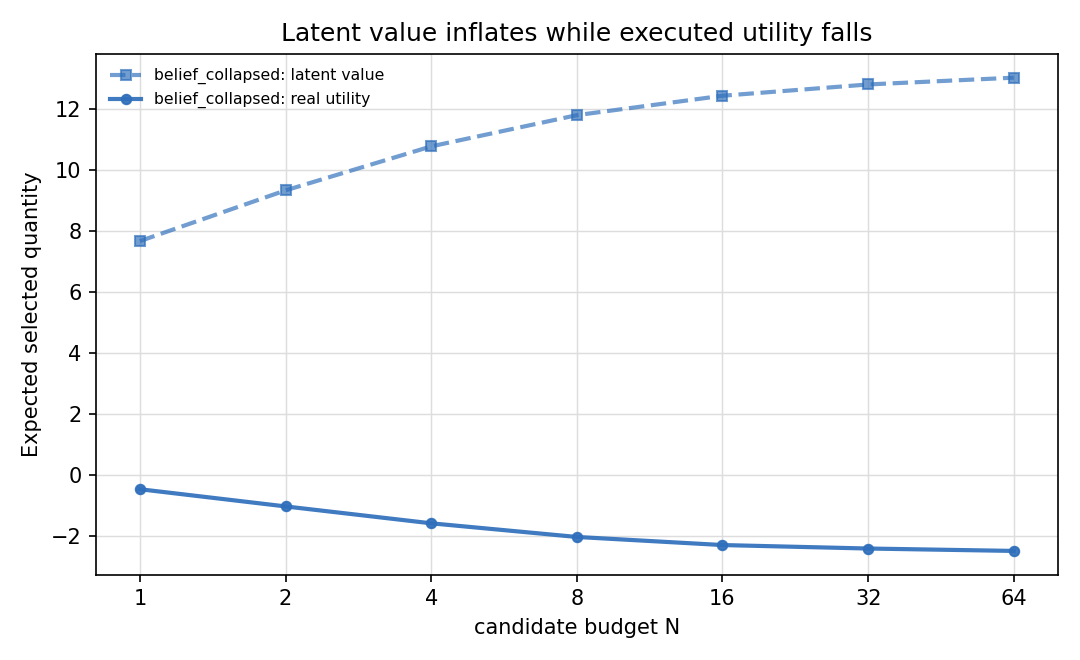
\includegraphics[width=0.78\linewidth]{figure1_latent_mismatch.png}
  \caption{Controlled and learned selected-tail mismatch. Raw latent selection can increase imagined selected value as \(N\) grows while selected executed utility falls or stalls.}
  \label{fig:mismatch-main}
\end{figure}

\paragraph{Belief collapse, horizon, and repairs.}
Experiment C isolates hidden-mode belief collapse. Raw large-budget selection concentrates in optimistic imagined modes: the selected tail has imagined free probability \(0.964\) while \(72.5\%\) of selected candidates execute in blocked modes, and real utility drops by \(1.34\) from \(N=1\) to \(N=64\). Experiment D varies horizon and selection budget. At horizon \(H=8\), raw selected latent value rises by \(10.99\), selected real utility drops by \(4.10\), and the combined repair improves \(N=64\) real utility by \(9.44\). Experiment E compares repairs directly: combined repair improves \(N=64\) real utility by \(5.05\) over raw and closes \(65.7\%\) of the raw-to-oracle gap.

\paragraph{Belief-intervention stress.}
Experiment J attacks the mechanism directly across 20 high-risk seed-regime units. Raw high-\(N\) selection is harmful in 18 of 20 units: selected latent value rises by \(6.88\), while selected real utility changes by \(-2.28\) with bootstrap \(\mathrm{CI}=[-2.99,-1.52]\). A diagnostic-only posterior-prior plus belief-collapse penalty improves \(N=64\) selected real utility over raw by \(3.11\) (\(\mathrm{CI}=[2.68,3.54]\)) without using pilot labels. Pilot calibration plus the full diagnostic penalty improves by \(5.83\) (\(\mathrm{CI}=[4.87,6.89]\)), while oracle remains \(4.06\) higher (\(\mathrm{CI}=[3.61,4.57]\)). The raw selected tail's posterior-prior/belief drift correlates with latent-real gap at \(0.401\) (\(\mathrm{CI}=[0.361,0.444]\)). This supports the RSSM-specific diagnosis without claiming that the repair reaches oracle selection.

\begin{figure}[t]
  \centering
  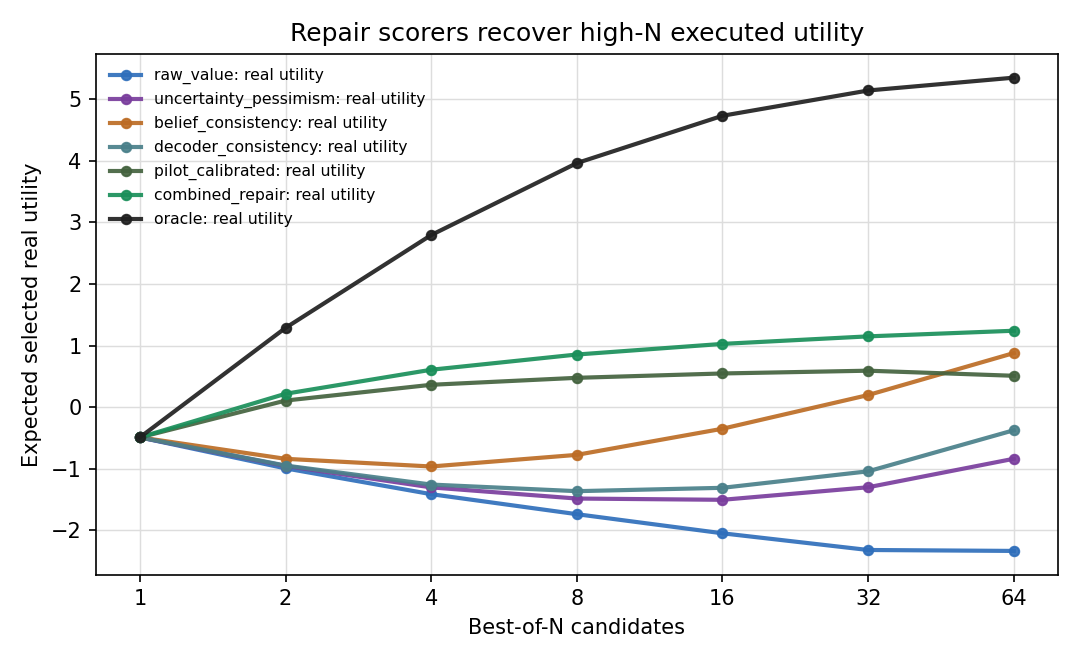
\includegraphics[width=0.82\linewidth]{figure2_repair_comparison.png}
  \caption{Repair comparison in the controlled setting. Pilot calibration plus conservative \rssm-style penalties recovers much of the selected-tail utility, but the oracle remains above the repaired scorer.}
  \label{fig:repair-main}
\end{figure}

\paragraph{Closed-loop and label-budget evidence.}
In receding-horizon planning (Experiment F), raw large-budget selection underperforms both oracle and repair. In the controlled planner, raw \(N=64\) mean return is \(-3.08\), compared with raw \(N=1\) at \(-0.98\), combined repair at \(0.77\), and oracle at \(1.90\). In the learned planner, raw \(N=64\) is \(-1.26\), raw \(N=1\) is \(-0.19\), combined repair is \(0.97\), and oracle is \(2.62\). Experiment G shows that pilot calibration does not require evaluation leakage: with five seeds, 16 labels improve \(N=64\) utility by \(3.31\) over raw, 128 labels by \(3.97\), and 1000 labels by \(4.30\), closing \(57.1\%\) of the raw-to-oracle gap.

\paragraph{OOD regimes and standard Gymnasium benchmarks.}
Experiment H sweeps hidden-mode probability, clue strength, and horizon. Raw large-budget selection is harmful in 30 of 36 regimes, neutral in 1, and helpful in 5; combined repair reduces average harm in high-risk regions by \(5.29\). This heterogeneity is important: the claim is not that large \(N\) is intrinsically bad. Experiment I adds exactly three Gymnasium toy-text benchmarks \citep{towers2024gymnasium}. Selected-tail mismatch appears in CliffWalkingSlippery and Taxi but not materially in FrozenLake. Combined repair improves \(N=64\) utility on all three, with large gains on the two mismatch benchmarks (Table~\ref{tab:gym-main}).

Experiment K adds three standard Gymnasium classic-control tasks with low-dimensional continuous dynamics: CartPole-v1, MountainCar-v0, and Acrobot-v1. Candidate action sequences are selected by a biased optimistic latent proxy and then executed in the real benchmark environment. Raw high-\(N\) selection increases selected latent value and risk in all three tasks. It hurts executed utility in CartPole and Acrobot, where combined RSSM diagnostics improve \(N=64\) utility with positive bootstrap lower bounds; MountainCar is a boundary case where raw high-\(N\) selection helps, preventing a universal-harm claim (Table~\ref{tab:classic-control-main}). These Gymnasium results are standard low-dimensional stress tests, not full Dreamer benchmark coverage.

\begin{table}[t]
\centering
\caption{Gymnasium toy-text benchmark summary. Values are mean executed utility; higher is better.}
\label{tab:gym-main}
\begin{tabular}{lrrrr}
\toprule
Benchmark & Raw \(N=1\) & Raw \(N=64\) & Repair \(N=64\) & Oracle \(N=64\) \\
\midrule
FrozenLake-v1 & 0.02 & 0.01 & 0.01 & 0.03 \\
CliffWalkingSlippery-v1 & -206.24 & -253.61 & -124.37 & -124.37 \\
Taxi-v3 & -53.17 & -85.97 & -19.94 & -19.93 \\
\bottomrule
\end{tabular}
\end{table}

\begin{table}[t]
\centering
\caption{Classic-control benchmark effects. Values are seed-level means with 95\% bootstrap intervals in brackets. Latent \(\Delta\) and real \(\Delta\) are raw \(N=64\) minus raw \(N=1\); repair gain is combined repair \(N=64\) minus raw \(N=64\).}
\label{tab:classic-control-main}
\begin{tabular}{lrrr}
\toprule
Benchmark & Raw latent \(\Delta\) & Raw real \(\Delta\) & Repair gain \\
\midrule
CartPole-v1 & \(17.59\,[16.55,18.42]\) & \(-1.15\,[-1.76,-0.67]\) & \(11.73\,[8.79,15.48]\) \\
Acrobot-v1 & \(20.80\,[19.83,21.86]\) & \(-1.81\,[-2.12,-1.59]\) & \(2.80\,[1.55,4.13]\) \\
MountainCar-v0 & \(33.72\,[31.51,35.59]\) & \(5.10\,[4.21,5.89]\) & \(0.00\,[0.00,0.00]\) \\
\bottomrule
\end{tabular}
\end{table}

\section{Related Work}

RSSM world models were introduced for latent planning from pixels in PlaNet and developed into Dreamer-style latent imagination agents \citep{hafner2019planet,hafner2020dreamer,hafner2021dreamerv2,hafner2023dreamerv3}. Model-based RL more broadly has long used learned dynamics for planning and policy improvement \citep{deisenroth2011pilco,chua2018pets,janner2019mbpo}. A recurring concern is model exploitation: optimizing against an imperfect learned model can find trajectories that look good to the model but execute poorly \citep{talvitie2017selfcorrecting}. Conservative model-based methods and uncertainty-aware penalties address related risks, especially in offline or limited-data settings \citep{kidambi2020morel,yu2020mopo}.

Candidate reranking and reward-model selection are also common outside RL, including human-feedback systems that sample multiple outputs and select with a learned reward model \citep{stiennon2020summarize,nakano2021webgpt,gao2023overoptimization}. Our finite estimator is an empirical order-statistic identity \citep{david2003orderstatistics}, but the application here is \rssm-style latent planning where score, diagnostics, and executed utility are all separately observable. Calibration work \citep{guo2017calibration} motivates our pilot-calibrated repair, while ensemble and dropout uncertainty methods motivate uncertainty diagnostics \citep{gal2016dropout,lakshminarayanan2017ensembles}. The contribution is not a new world-model architecture; it is a measurement and diagnostic protocol for selected-tail latent-real mismatch.

\section{Limitations}

The evidence is intentionally bounded. The learned model is small and CPU-trained. The controlled environments are hidden-mode toys designed to make latent-real mismatch inspectable. The Gymnasium benchmarks are three lightweight toy-text stochastic tasks and three standard classic-control tasks with low-dimensional states. We do not evaluate a full Dreamer implementation, a broad model-based RL benchmark suite, real robots, safety-critical deployment, or high-dimensional visual-control domains. The repair scorers are diagnostic baselines, not a universal recipe; their relative performance varies across settings. Finally, high \(N\) is sometimes neutral or helpful in the OOD grid and MountainCar, so the correct conclusion is conditional: selection amplifies the upper-tail relationship between model score and executed utility.

\section{Reproducibility Statement}

The supplementary source contains scripts that regenerate all JSON, CSV, figure, and audit artifacts. The publication-style checks are \texttt{bash scripts/run\_all.sh}, \texttt{bash scripts/run\_claim\_audit.sh}, and \texttt{pytest}. The appendix gives the estimator proof, experimental configurations, all figures, leakage audit details, and claim boundaries. The anonymous submission PDF is built from this directory with standard \texttt{pdflatex}/\texttt{bibtex} passes.

\bibliographystyle{iclr2026_conference}
\bibliography{references}

\appendix
\section{Proof Details}
\label{app:proof}

For a tie group \(g\), the event that the maximum sampled score falls in \(g\) occurs when every draw has rank at most \(r_g^{\max}\) and at least one draw has rank at least \(r_g^{\min}\). Since each draw is uniform over the \(m\) candidates and sampling is with replacement, this probability is
\[
\left(\frac{r_g^{\max}}{m}\right)^N -
\left(\frac{r_g^{\min}-1}{m}\right)^N.
\]
Conditional on this event, all sampled candidates with the maximum score are members of the same tie group. Uniform tie-breaking among the top-score sampled candidates gives the group mean measured utility \(\bar{\utility}_g\). Summing over the disjoint score groups yields Equation~\ref{eq:tail-estimator}.

For binary utility and \(N=2\), let \(p=P(\utility=1)\) in the empirical pool and let \(\kappa=P(\score^+>\score^-)+0.5P(\score^+=\score^-)\), the tie-aware AUC. Two successes select success with probability \(p^2\). One success and one failure occur with probability \(2p(1-p)\), and the success is selected with probability \(\kappa\). Thus \(f_2=p^2+2p(1-p)\kappa\), matching the implementation check.

\section{Additional Figures}

\begin{figure}[t]
  \centering
  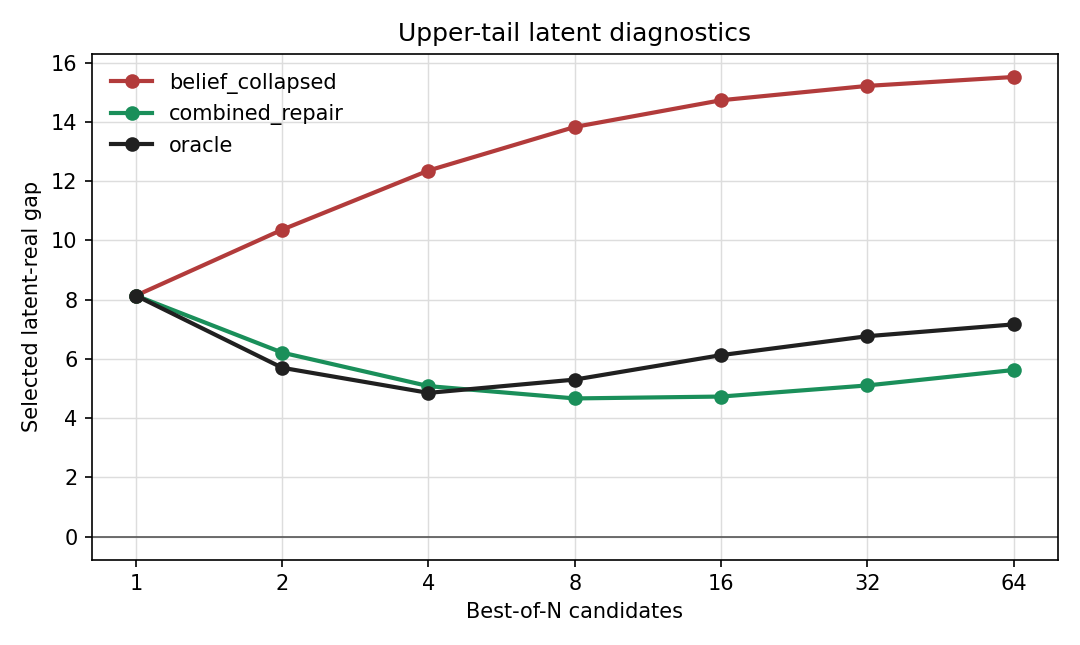
\includegraphics[width=0.82\linewidth]{figure3_tail_diagnostics.png}
  \caption{Selected-tail diagnostics. High raw latent value is associated with larger latent-real gaps, high imagined free probability, and adverse executed modes in the controlled setting.}
  \label{fig:tail-appendix}
\end{figure}

\begin{figure}[t]
  \centering
  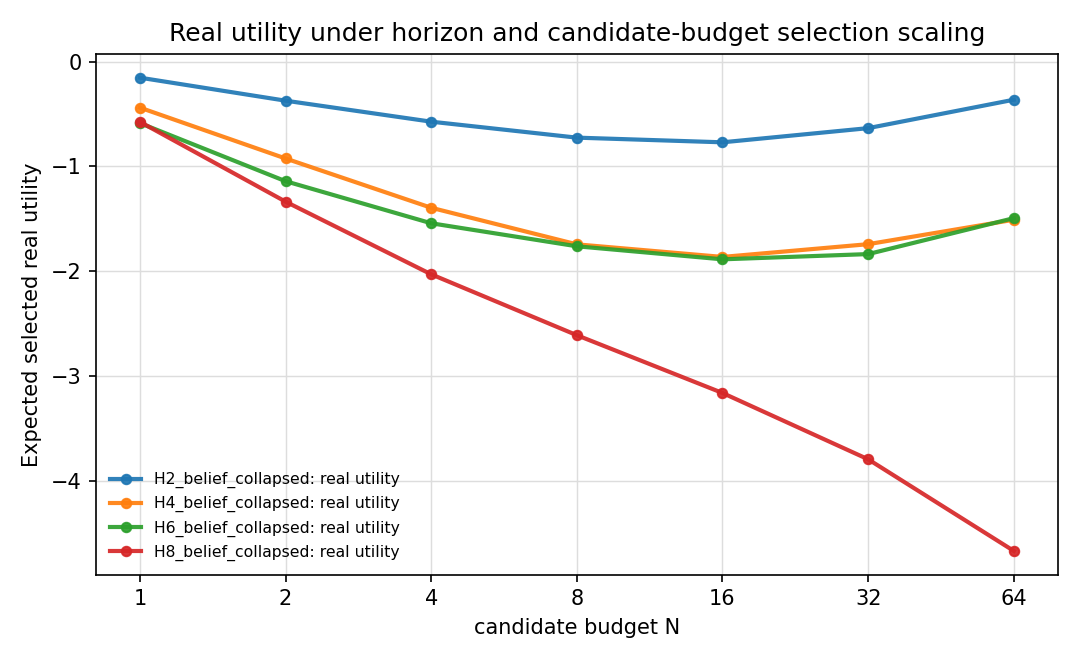
\includegraphics[width=0.82\linewidth]{figure4_horizon_budget.png}
  \caption{Horizon and selection-budget sweep. Longer horizons can make the selected latent-real mismatch larger under optimistic latent scoring.}
  \label{fig:horizon-appendix}
\end{figure}

\begin{figure}[t]
  \centering
  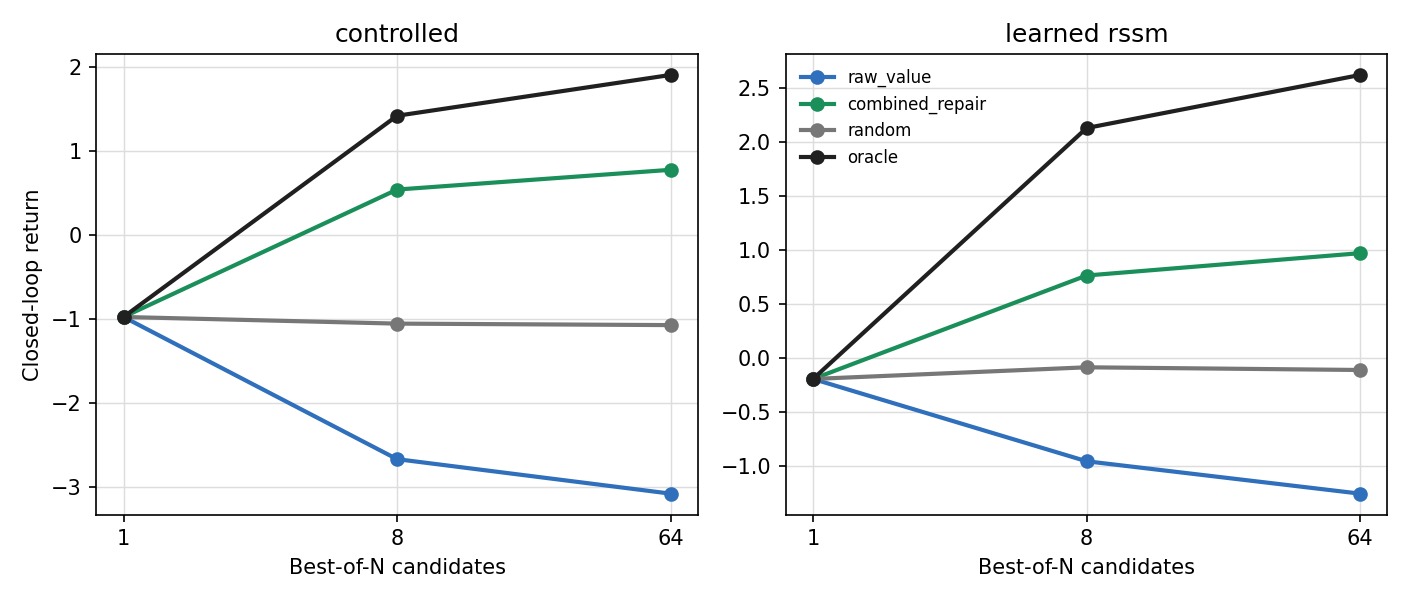
\includegraphics[width=0.82\linewidth]{figure6_closed_loop_planning.png}
  \caption{Closed-loop receding-horizon planning in controlled and learned \rssm-style settings. Raw large-budget planning underperforms repair and oracle.}
  \label{fig:closed-loop-appendix}
\end{figure}

\begin{figure}[t]
  \centering
  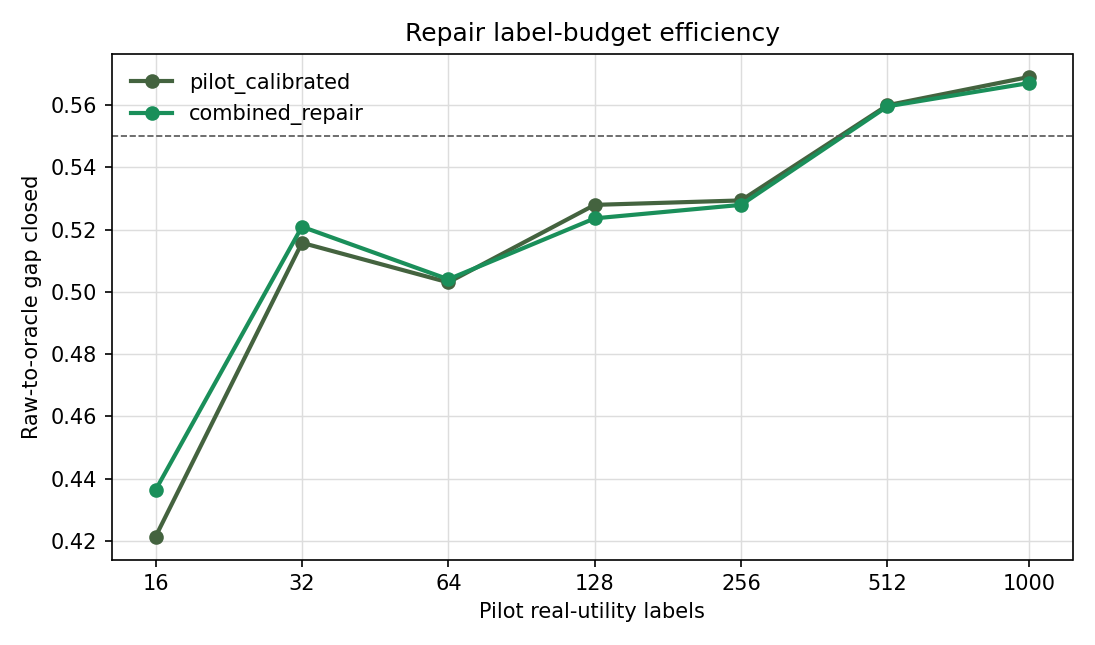
\includegraphics[width=0.82\linewidth]{figure7_label_budget_repair.png}
  \caption{Pilot-label budget ablation. Small disjoint pilot sets already improve selected-tail utility; larger budgets recover more of the raw-to-oracle gap.}
  \label{fig:label-budget-appendix}
\end{figure}

\begin{figure}[t]
  \centering
  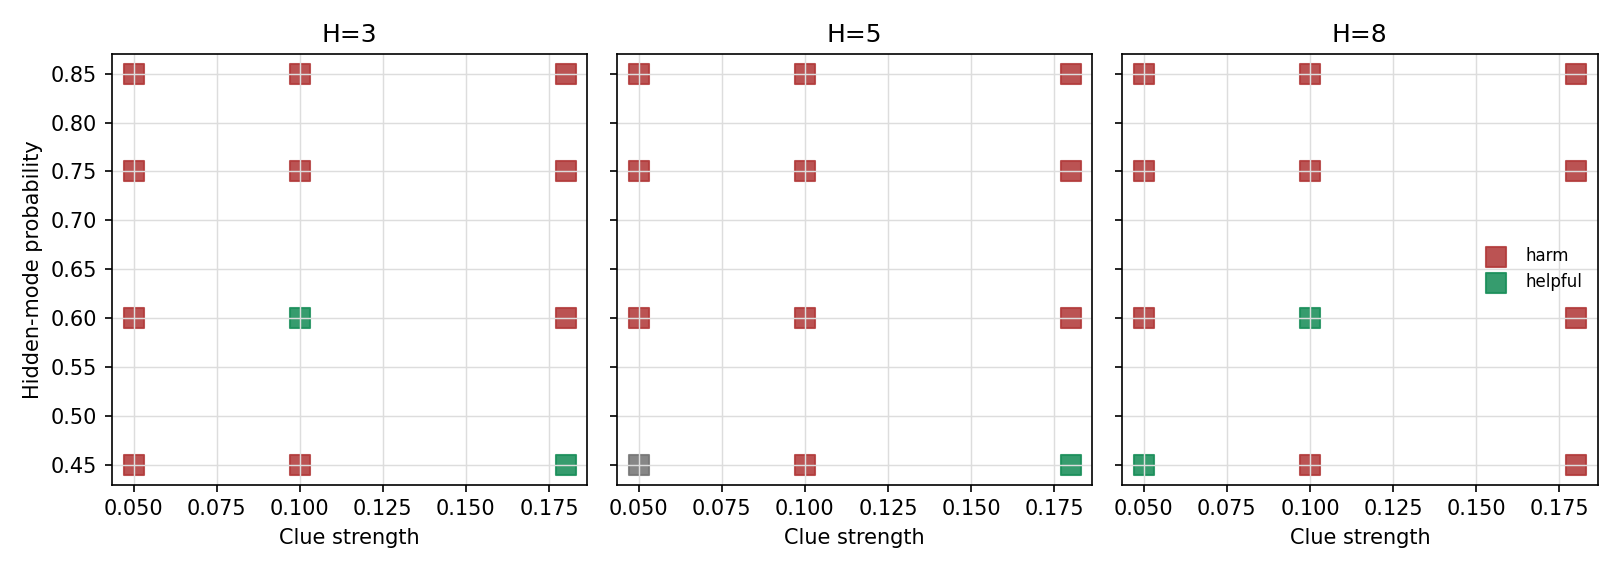
\includegraphics[width=0.82\linewidth]{figure8_ood_stress_grid.png}
  \caption{OOD stress grid over hidden-mode probability, clue strength, and horizon. Raw large-budget selection is harmful in many regimes but can be neutral or helpful in others.}
  \label{fig:ood-appendix}
\end{figure}

\begin{figure}[t]
  \centering
  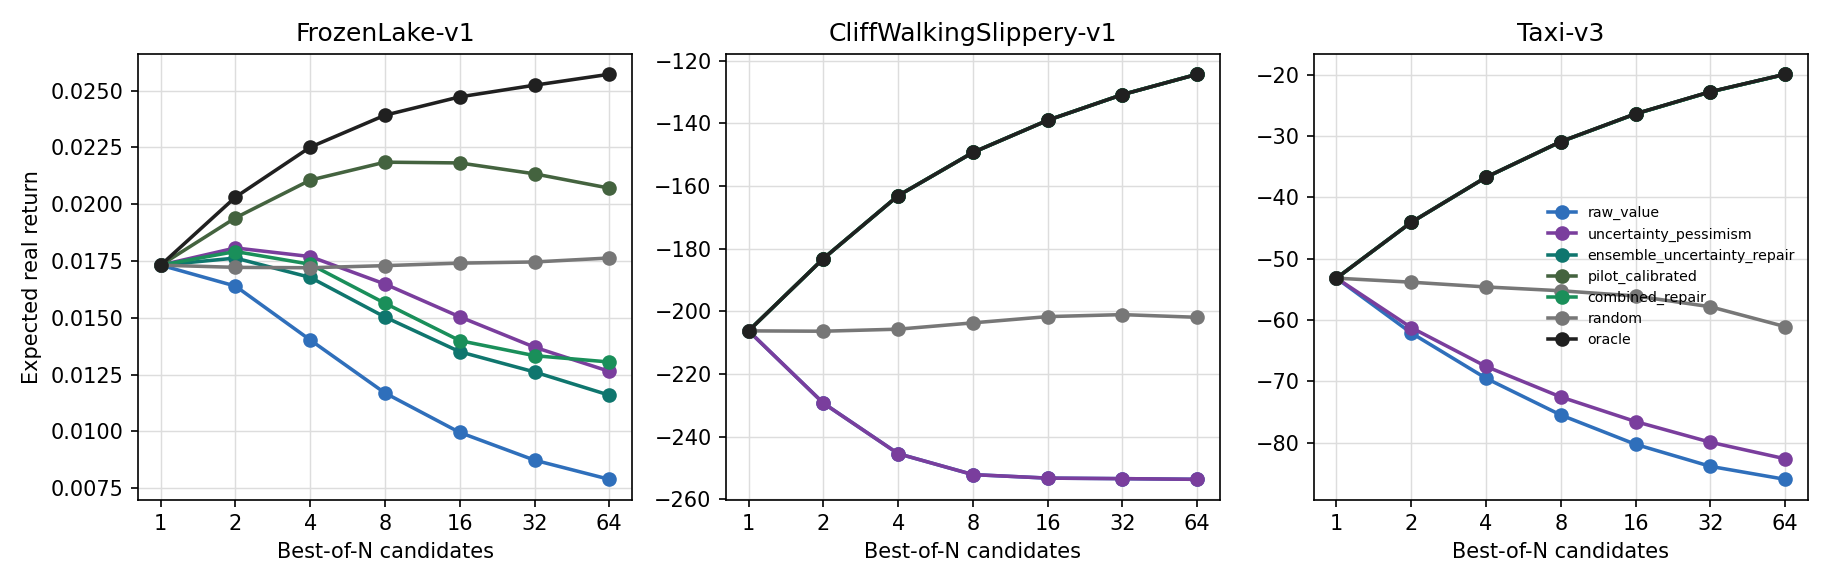
\includegraphics[width=0.82\linewidth]{figure9_gymnasium_benchmarks.png}
  \caption{Three lightweight Gymnasium toy-text benchmarks. Mismatch is pronounced in CliffWalkingSlippery and Taxi, minimal in FrozenLake, and repair improves \(N=64\) utility on all three.}
  \label{fig:gym-appendix}
\end{figure}

\begin{figure}[t]
  \centering
  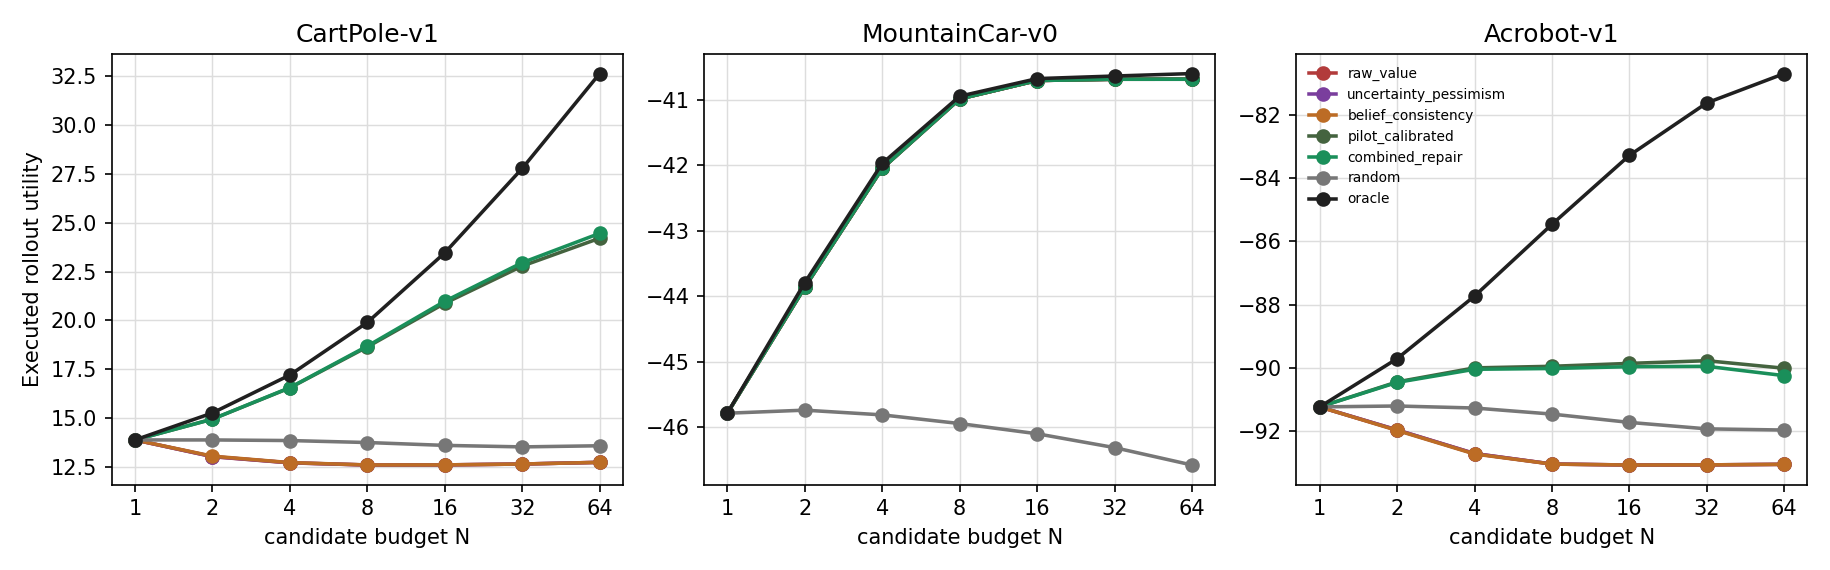
\includegraphics[width=0.82\linewidth]{figure11_classic_control_benchmarks.png}
  \caption{Three standard Gymnasium classic-control tasks. CartPole and Acrobot expose optimistic latent-tail failure and repair recovery; MountainCar is a boundary case where raw high-\(N\) selection is helpful.}
  \label{fig:classic-control-appendix}
\end{figure}

\begin{figure}[t]
  \centering
  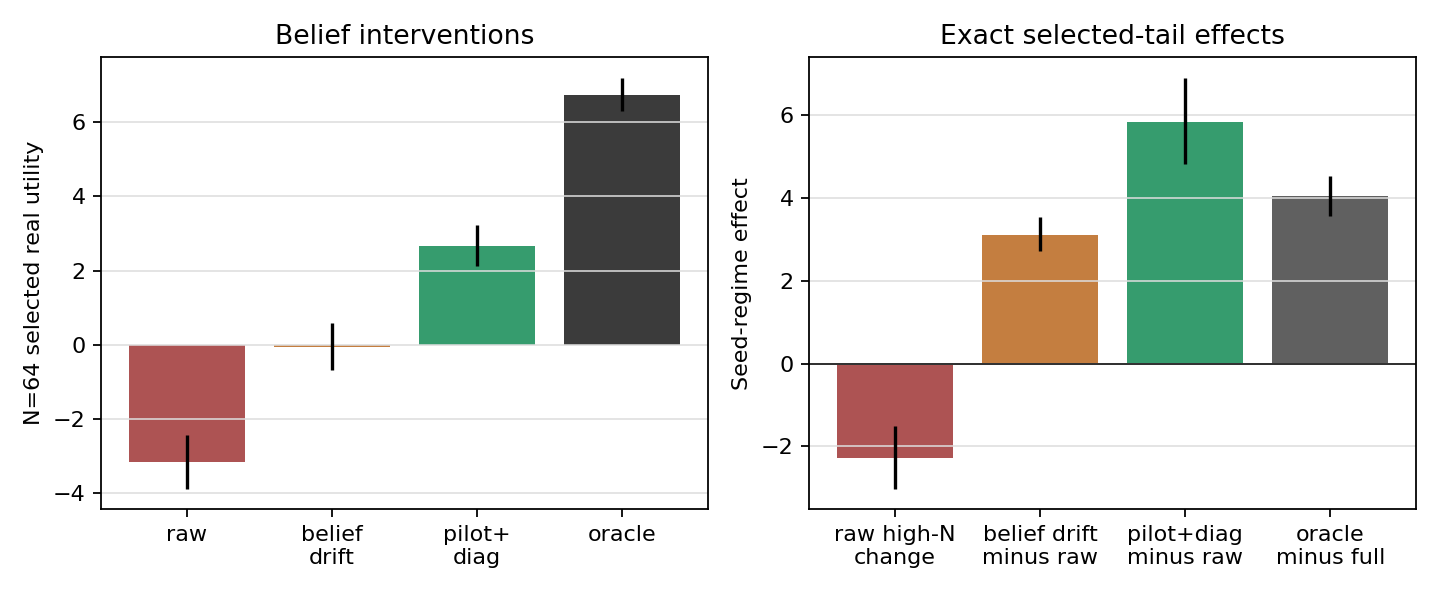
\includegraphics[width=0.82\linewidth]{figure10_belief_interventions.png}
  \caption{Belief-intervention stress. Posterior-prior and belief-collapse penalties recover selected-tail real utility in high-risk RSSM-style regimes, but the oracle gap remains visible.}
  \label{fig:belief-intervention-appendix}
\end{figure}

\section{Experiment Configurations and Artifacts}

All result files are generated by the scripts in the supplementary source. The main artifacts are:
\begin{itemize}
  \item selected-tail estimator validation: \path{results/selected_tail_estimator_validation.json};
  \item controlled latent mismatch: \path{results/experiment_a_toy_mismatch.json};
  \item learned \rssm-style model: \path{results/experiment_b_learned_rssm.json} and \path{results/learned_tiny_rssm.pt};
  \item belief collapse and horizon sweeps: \path{results/experiment_c_belief_collapse.json} and \path{results/experiment_d_horizon_budget.json};
  \item repair, belief intervention, closed-loop, and label-budget studies: \path{results/experiment_e_repairs.json}, \path{results/experiment_j_belief_interventions.json}, \path{results/experiment_f_closed_loop_planning.json}, and \path{results/experiment_g_label_budget_ablation.json};
  \item OOD and Gymnasium studies: \path{results/experiment_h_ood_stress_grid.json}, \path{results/experiment_i_gymnasium_benchmarks.json}, and \path{results/experiment_k_classic_control_benchmarks.json};
  \item claim and leakage audits: \path{results/claims_status.json} and \path{results/leakage_audit.json}.
\end{itemize}

The strict multiseed audit reports strong evidence for the controlled latent dynamics family over five seeds: mean raw latent delta \(5.41\), mean raw real delta \(-1.98\), and mean repair improvement \(6.20\). The learned \rssm-style family uses three seeds: mean raw latent delta \(0.96\), mean raw real delta \(-1.64\), and mean repair improvement \(5.30\). The belief-intervention stress adds 20 seed-regime units with raw high-\(N\) harm in \(90\%\) of units and positive posterior-prior diagnostic recovery. The classic-control tier contributes 3,240 executed Gymnasium rollout records and 18 seed-benchmark effect rows; two of three tasks meet mismatch and repair thresholds, while MountainCar is a declared helpful-boundary case. These summaries support the qualitative claims while preserving the small-scale scope of the evidence.

\section{Leakage Audit and Boundary Cases}

Pilot calibration uses real-utility labels only from the pilot split. Evaluation candidates may be scored by the fitted calibrator, but their labels are used only after scoring for reporting selected utility. The audit verifies zero pilot/evaluation overlap and zero leaked labels for clean runs. A sentinel run deliberately inserts three non-pilot evaluation labels into calibrator provenance; the audit rejects it with reasons that the calibrator labels include non-pilot candidates and that label provenance is not a subset of the pilot split.

Boundary cases are reviewer-facing sanity checks. Constant utility remains constant for every \(N\). Oracle scoring \(S=R\) improves selected utility with \(N\) in the finite pool. Anti-aligned scoring \(S=-R\) worsens selected utility. The OOD grid and MountainCar benchmark include regimes where raw large-budget selection is neutral or helpful. These cases are important because the paper's claim is conditional on latent-real selected-tail mismatch rather than a blanket statement about selection budgets.

\end{document}
